\documentclass[border=5pt]{standalone}
% Shared by every figure. Colour marks the TYPE of a quantity, never decoration:
%   blue   (vec) equivariant: rotates with its fragment     -- solid arrows
%   orange (inv) invariant: unchanged by any rotation        -- dashed arrows
%   aqua   (att) attention / communication between elements
%   violet (out) what the network outputs
% Text is always ink; a coloured mark next to it carries the meaning.
\usepackage{amsmath,amssymb,bm}
\usepackage{tikz}
\usetikzlibrary{arrows.meta,positioning,fit,backgrounds,calc,shapes.geometric,
  shapes.misc,decorations.pathreplacing,decorations.pathmorphing,matrix,
  patterns,cd,shadows}
\definecolor{vec}{HTML}{2A78D6}
\definecolor{inv}{HTML}{EB6834}
\definecolor{att}{HTML}{1BAF7A}
\definecolor{out}{HTML}{4A3AA7}
\definecolor{ink}{HTML}{0B0B0B}
\definecolor{ink2}{HTML}{52514E}
\definecolor{ink3}{HTML}{8A877F}
\definecolor{neutral}{HTML}{F0EFEC}
\definecolor{rule}{HTML}{CFCCC4}
\definecolor{pieceA}{HTML}{E4E1DA}
\definecolor{pieceB}{HTML}{CDC9BF}
\definecolor{pieceC}{HTML}{B3AEA2}
\colorlet{vecfill}{vec!9}
\colorlet{invfill}{inv!10}
\colorlet{attfill}{att!11}
\colorlet{outfill}{out!9}
\tikzset{
  >={Stealth[length=2.3mm,width=1.7mm]},
  every picture/.style={line cap=round, line join=round},
  box/.style={draw=ink2, fill=neutral, rounded corners=2.5pt, align=center,
    font=\small, inner sep=4pt, minimum height=8mm, text=ink, line width=0.6pt, nohyph},
  vecbox/.style={box, draw=vec, fill=vecfill},
  invbox/.style={box, draw=inv, fill=invfill},
  attbox/.style={box, draw=att, fill=attfill},
  outbox/.style={box, draw=out, fill=outfill},
  plain/.style={box, draw=ink3, fill=white},
  arr/.style={->, draw=ink2, line width=0.7pt},
  vecarr/.style={->, draw=vec, line width=1.1pt},
  invarr/.style={->, draw=inv, line width=1.1pt, dash pattern=on 3.2pt off 1.8pt},
  attarr/.style={->, draw=att, line width=1.1pt, dash pattern=on 1.2pt off 1.4pt},
  outarr/.style={->, draw=out, line width=1.1pt},
  nohyph/.style={execute at begin node={\hyphenpenalty=10000\exhyphenpenalty=10000\relax}},
  lbl/.style={font=\footnotesize, text=ink2, align=center, nohyph},
  tlbl/.style={font=\footnotesize, text=ink, align=center, nohyph},
  group/.style={draw=ink3, dashed, rounded corners=5pt, inner sep=7pt},
  op/.style={circle, draw=ink2, fill=white, inner sep=0pt, minimum size=5.2mm,
    font=\small, line width=0.6pt},
  piece/.style={fill=#1, draw=none},
  intact/.style={draw=ink2, line width=0.6pt},
  fracture/.style={draw=ink, line width=1.5pt},
  token/.style={circle, fill=att, draw=white, line width=0.5pt, inner sep=0pt,
    minimum size=4.2pt},
  vtx/.style={circle, fill=ink, inner sep=0pt, minimum size=3pt},
  panel/.style={font=\small\bfseries, text=ink, anchor=north west},
}
% one piece of the cartoon, in its own centred frame: fill, intact edge, fracture edge
\newcommand{\drawpiece}[2]{% #1 = A|B|C, #2 = fill colour
  \fill[#2] \csname Piece#1\endcsname;
  \draw[intact] \csname Intact#1\endcsname;
  \draw[fracture] \csname Crack#1\endcsname;}
% a legend entry: a short line in a given style, then its text
\newcommand{\legendline}[3]{% #1 position, #2 style, #3 text
  \draw[#2] (#1) -- ++(0.7,0) node[right, tlbl, text=ink] {#3};}

\begin{document}
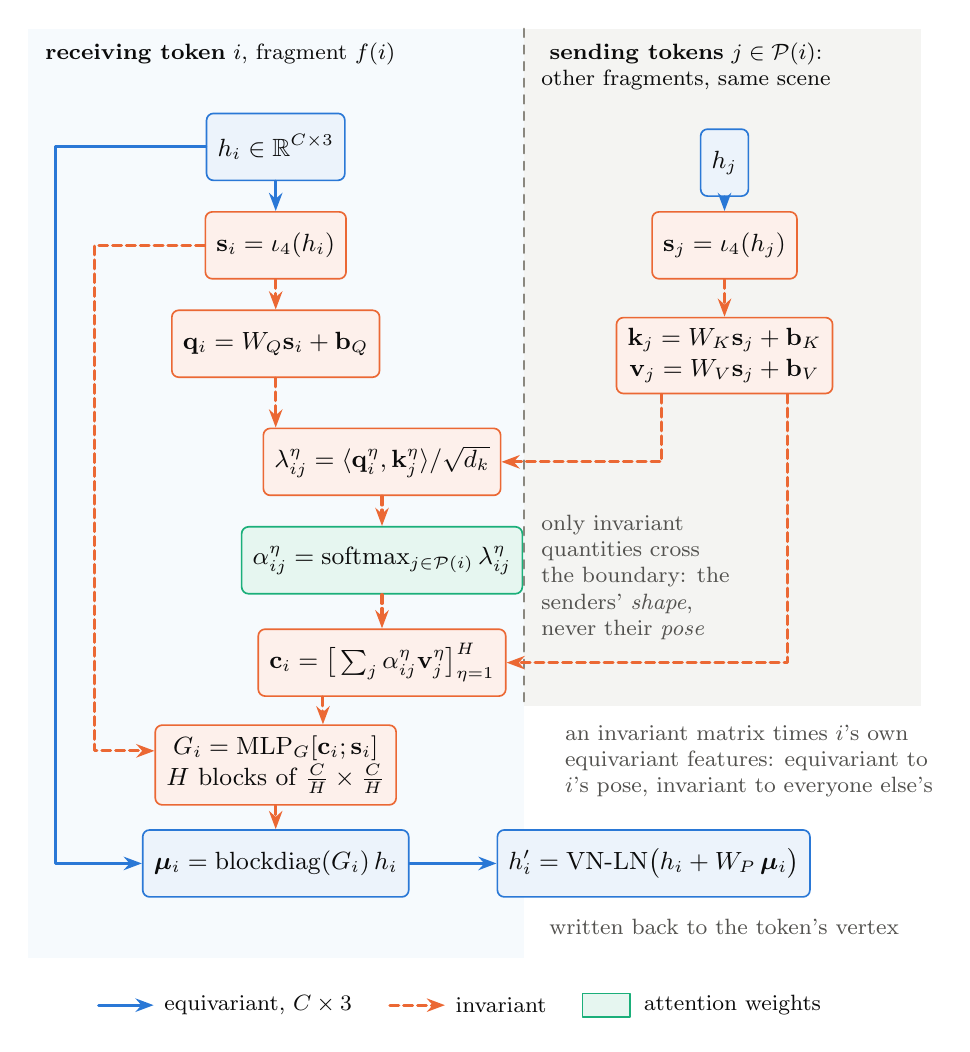
\begin{tikzpicture}
  \tikzset{fb/.style={font=\small, minimum height=8.5mm}, note/.style={lbl, align=left, anchor=west}}
  % sides
  \fill[vecfill!45] (-0.95,0.75) rectangle (5.35,-11.05);
  \fill[neutral!70] (5.35,0.75) rectangle (10.4,-7.85);
  \draw[ink3, dashed, line width=0.8pt] (5.35,0.75) -- (5.35,-7.85);
  \node[tlbl, anchor=north west] at (-0.85,0.7) {\textbf{receiving token} $i$, fragment $f(i)$};
  \node[tlbl, anchor=north west] at (5.45,0.7) {\textbf{sending tokens} $j\in\mathcal P(i)$:\\ other fragments, same scene};
  % inputs and invariant descriptions
  \node[vecbox, fb] (hi) at (2.2,-0.75) {$h_i\in\mathbb R^{C\times 3}$};
  \node[vecbox, fb] (hj) at (7.9,-0.95) {$h_j$};
  \node[invbox, fb] (si) at (2.2,-2.0) {$\mathbf s_i=\iota_4(h_i)$};
  \node[invbox, fb] (sj) at (7.9,-2.0) {$\mathbf s_j=\iota_4(h_j)$};
  \draw[vecarr] (hi) -- (si);
  \draw[vecarr] (hj) -- (sj);
  \node[invbox, fb] (qi) at (2.2,-3.25) {$\mathbf q_i=W_Q\mathbf s_i+\mathbf b_Q$};
  \node[invbox, fb, align=center] (kj) at (7.9,-3.4) {$\mathbf k_j=W_K\mathbf s_j+\mathbf b_K$\\ $\mathbf v_j=W_V\mathbf s_j+\mathbf b_V$};
  \draw[invarr] (si) -- (qi);
  \draw[invarr] (sj) -- (kj);
  % attention across the boundary
  \node[invbox, fb] (lam) at (3.55,-4.75) {$\lambda_{ij}^{\eta}=\langle\mathbf q_i^{\eta},\mathbf k_j^{\eta}\rangle/\sqrt{d_k}$};
  \draw[invarr] (qi) -- (qi |- lam.north);
  \draw[invarr] ($(kj.south)+(-0.8,0)$) |- (lam.east);
  \node[attbox, fb] (alp) at (3.55,-6.0) {$\alpha_{ij}^{\eta}=\mathrm{softmax}_{j\in\mathcal P(i)}\,\lambda_{ij}^{\eta}$};
  \draw[invarr] (lam) -- (alp);
  \node[invbox, fb] (ctx) at (3.55,-7.3) {$\mathbf c_i=\big[\textstyle\sum_{j}\alpha_{ij}^{\eta}\mathbf v_j^{\eta}\big]_{\eta=1}^{H}$};
  \draw[invarr] (alp) -- (ctx);
  \draw[invarr] ($(kj.south)+(0.8,0)$) |- (ctx.east);
  % the matrix-valued message
  \node[invbox, fb, align=center] (G) at (2.2,-8.6) {$G_i=\mathrm{MLP}_G[\mathbf c_i;\mathbf s_i]$\\ $H$ blocks of $\tfrac CH\times\tfrac CH$};
  \draw[invarr] (ctx.south -| G.north) ++(0.6,0) -- ($(G.north)+(0.6,0)$);
  \draw[invarr] (si.west) -- (-0.1,-2.0) |- ($(G.west)+(0,0.18)$);
  \node[vecbox, fb] (mu) at (2.2,-9.85) {$\boldsymbol\mu_i=\mathrm{blockdiag}(G_i)\,h_i$};
  \draw[invarr] (G) -- (mu);
  \draw[vecarr] (hi.west) -- (-0.6,-0.75) |- (mu.west);
  \node[vecbox, fb] (out) at (7.0,-9.85) {$h_i'=\mathrm{VN\text{-}LN}\big(h_i+W_P\,\boldsymbol\mu_i\big)$};
  \draw[vecarr] (mu) -- (out);
  \node[note] at (5.55,-10.65) {written back to the token's vertex};
  % notes
  \node[note, anchor=north west] at (5.45,-5.3) {only invariant\\ quantities cross\\ the boundary: the\\ senders' \emph{shape},\\ never their \emph{pose}};
  \node[note] at (5.75,-8.55) {an invariant matrix times $i$'s own\\ equivariant features: equivariant to\\ $i$'s pose, invariant to everyone else's};
  % legend
  \begin{scope}[shift={(7.55,-11.65)}]
    \draw[vecarr] (-7.6,0) -- (-6.9,0) node[right, tlbl] {equivariant, $C\times 3$};
    \draw[invarr] (-3.9,0) -- (-3.2,0) node[right, tlbl] {invariant};
    \fill[attfill, draw=att] (-1.45,-0.15) rectangle (-0.85,0.15);
    \node[right, tlbl] at (-0.8,0) {attention weights};
  \end{scope}
\end{tikzpicture}
\end{document}
